\documentclass[1p]{elsarticle_modified}
%\bibliographystyle{elsarticle-num}

%\usepackage[colorlinks]{hyperref}
%\usepackage{abbrmath_seonhwa} %\Abb, \Ascr, \Acal ,\Abf, \Afrak
\usepackage{amsfonts}
\usepackage{amssymb}
\usepackage{amsmath}
\usepackage{amsthm}
\usepackage{scalefnt}
\usepackage{amsbsy}
\usepackage{kotex}
\usepackage{caption}
\usepackage{subfig}
\usepackage{color}
\usepackage{graphicx}
\usepackage{xcolor} %% white, black, red, green, blue, cyan, magenta, yellow
\usepackage{float}
\usepackage{setspace}
\usepackage{hyperref}

\usepackage{tikz}
\usetikzlibrary{arrows}

\usepackage{multirow}
\usepackage{array} % fixed length table
\usepackage{hhline}

%%%%%%%%%%%%%%%%%%%%%
\makeatletter
\renewcommand*\env@matrix[1][\arraystretch]{%
	\edef\arraystretch{#1}%
	\hskip -\arraycolsep
	\let\@ifnextchar\new@ifnextchar
	\array{*\c@MaxMatrixCols c}}
\makeatother %https://tex.stackexchange.com/questions/14071/how-can-i-increase-the-line-spacing-in-a-matrix
%%%%%%%%%%%%%%%

\usepackage[normalem]{ulem}

\newcommand{\msout}[1]{\ifmmode\text{\sout{\ensuremath{#1}}}\else\sout{#1}\fi}
%SOURCE: \msout is \stkout macro in https://tex.stackexchange.com/questions/20609/strikeout-in-math-mode

\newcommand{\cancel}[1]{
	\ifmmode
	{\color{red}\msout{#1}}
	\else
	{\color{red}\sout{#1}}
	\fi
}

\newcommand{\add}[1]{
	{\color{blue}\uwave{#1}}
}

\newcommand{\replace}[2]{
	\ifmmode
	{\color{red}\msout{#1}}{\color{blue}\uwave{#2}}
	\else
	{\color{red}\sout{#1}}{\color{blue}\uwave{#2}}
	\fi
}

\newcommand{\Sol}{\mathcal{S}} %segment
\newcommand{\D}{D} %diagram
\newcommand{\A}{\mathcal{A}} %arc


%%%%%%%%%%%%%%%%%%%%%%%%%%%%%5 test

\def\sl{\operatorname{\textup{SL}}(2,\Cbb)}
\def\psl{\operatorname{\textup{PSL}}(2,\Cbb)}
\def\quan{\mkern 1mu \triangleright \mkern 1mu}

\theoremstyle{definition}
\newtheorem{thm}{Theorem}[section]
\newtheorem{prop}[thm]{Proposition}
\newtheorem{lem}[thm]{Lemma}
\newtheorem{ques}[thm]{Question}
\newtheorem{cor}[thm]{Corollary}
\newtheorem{defn}[thm]{Definition}
\newtheorem{exam}[thm]{Example}
\newtheorem{rmk}[thm]{Remark}
\newtheorem{alg}[thm]{Algorithm}

\newcommand{\I}{\sqrt{-1}}
\begin{document}

%\begin{frontmatter}
%
%\title{Boundary parabolic representations of knots up to 8 crossings}
%
%%% Group authors per affiliation:
%\author{Yunhi Cho} 
%\address{Department of Mathematics, University of Seoul, Seoul, Korea}
%\ead{yhcho@uos.ac.kr}
%
%
%\author{Seonhwa Kim} %\fnref{s_kim}}
%\address{Center for Geometry and Physics, Institute for Basic Science, Pohang, 37673, Korea}
%\ead{ryeona17@ibs.re.kr}
%
%\author{Hyuk Kim}
%\address{Department of Mathematical Sciences, Seoul National University, Seoul 08826, Korea}
%\ead{hyukkim@snu.ac.kr}
%
%\author{Seokbeom Yoon}
%\address{Department of Mathematical Sciences, Seoul National University, Seoul, 08826,  Korea}
%\ead{sbyoon15@snu.ac.kr}
%
%\begin{abstract}
%We find all boundary parabolic representation of knots up to 8 crossings.
%
%\end{abstract}
%\begin{keyword}
%    \MSC[2010] 57M25 
%\end{keyword}
%
%\end{frontmatter}

%\linenumbers
%\tableofcontents
%
\newcommand\colored[1]{\textcolor{white}{\rule[-0.35ex]{0.8em}{1.4ex}}\kern-0.8em\color{red} #1}%
%\newcommand\colored[1]{\textcolor{white}{ #1}\kern-2.17ex	\textcolor{white}{ #1}\kern-1.81ex	\textcolor{white}{ #1}\kern-2.15ex\color{red}#1	}

{\Large $\underline{12a_{0996}~(K12a_{0996})}$}

\setlength{\tabcolsep}{10pt}
\renewcommand{\arraystretch}{1.6}
\vspace{1cm}\begin{tabular}{m{100pt}>{\centering\arraybackslash}m{274pt}}
\multirow{5}{120pt}{
	\centering
	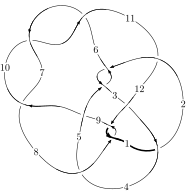
\includegraphics[width=112pt]{../../../GIT/diagram.site/Diagrams/png/1797_12a_0996.png}\\
\ \ \ A knot diagram\footnotemark}&
\allowdisplaybreaks
\textbf{Linearized knot diagam} \\
\cline{2-2}
 &
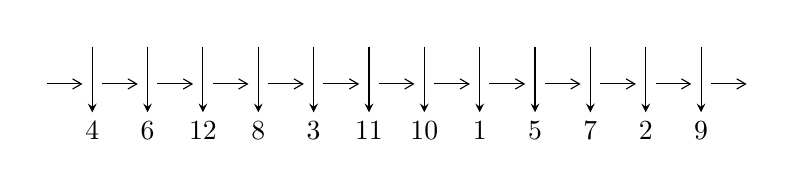
\begin{tikzpicture}[x=20pt, y=17pt]
	% nodes
	\node (C0) at (0, 0) {};
	\node (C1) at (1, 0) {};
	\node (C1U) at (1, +1) {};
	\node (C1D) at (1, -1) {4};

	\node (C2) at (2, 0) {};
	\node (C2U) at (2, +1) {};
	\node (C2D) at (2, -1) {6};

	\node (C3) at (3, 0) {};
	\node (C3U) at (3, +1) {};
	\node (C3D) at (3, -1) {12};

	\node (C4) at (4, 0) {};
	\node (C4U) at (4, +1) {};
	\node (C4D) at (4, -1) {8};

	\node (C5) at (5, 0) {};
	\node (C5U) at (5, +1) {};
	\node (C5D) at (5, -1) {3};

	\node (C6) at (6, 0) {};
	\node (C6U) at (6, +1) {};
	\node (C6D) at (6, -1) {11};

	\node (C7) at (7, 0) {};
	\node (C7U) at (7, +1) {};
	\node (C7D) at (7, -1) {10};

	\node (C8) at (8, 0) {};
	\node (C8U) at (8, +1) {};
	\node (C8D) at (8, -1) {1};

	\node (C9) at (9, 0) {};
	\node (C9U) at (9, +1) {};
	\node (C9D) at (9, -1) {5};

	\node (C10) at (10, 0) {};
	\node (C10U) at (10, +1) {};
	\node (C10D) at (10, -1) {7};

	\node (C11) at (11, 0) {};
	\node (C11U) at (11, +1) {};
	\node (C11D) at (11, -1) {2};

	\node (C12) at (12, 0) {};
	\node (C12U) at (12, +1) {};
	\node (C12D) at (12, -1) {9};
	\node (C13) at (13, 0) {};

	% arrows
	\draw[->,>={angle 60}]
	(C0) edge (C1) (C1) edge (C2) (C2) edge (C3) (C3) edge (C4) (C4) edge (C5) (C5) edge (C6) (C6) edge (C7) (C7) edge (C8) (C8) edge (C9) (C9) edge (C10) (C10) edge (C11) (C11) edge (C12) (C12) edge (C13) ;	\draw[->,>=stealth]
	(C1U) edge (C1D) (C2U) edge (C2D) (C3U) edge (C3D) (C4U) edge (C4D) (C5U) edge (C5D) (C6U) edge (C6D) (C7U) edge (C7D) (C8U) edge (C8D) (C9U) edge (C9D) (C10U) edge (C10D) (C11U) edge (C11D) (C12U) edge (C12D) ;
	\end{tikzpicture} \\
\hhline{~~} \\& 
\textbf{Solving Sequence} \\ \cline{2-2} 
 &
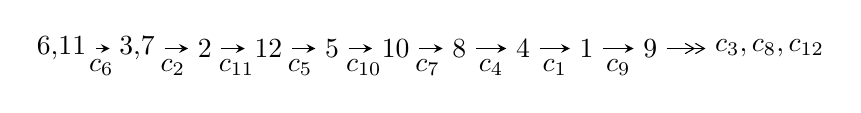
\begin{tikzpicture}[x=23pt, y=7pt]
	% node
	\node (A0) at (-1/8, 0) {6,11};
	\node (A1) at (17/16, 0) {3,7};
	\node (A2) at (17/8, 0) {2};
	\node (A3) at (25/8, 0) {12};
	\node (A4) at (33/8, 0) {5};
	\node (A5) at (41/8, 0) {10};
	\node (A6) at (49/8, 0) {8};
	\node (A7) at (57/8, 0) {4};
	\node (A8) at (65/8, 0) {1};
	\node (A9) at (73/8, 0) {9};
	\node (C1) at (1/2, -1) {$c_{6}$};
	\node (C2) at (13/8, -1) {$c_{2}$};
	\node (C3) at (21/8, -1) {$c_{11}$};
	\node (C4) at (29/8, -1) {$c_{5}$};
	\node (C5) at (37/8, -1) {$c_{10}$};
	\node (C6) at (45/8, -1) {$c_{7}$};
	\node (C7) at (53/8, -1) {$c_{4}$};
	\node (C8) at (61/8, -1) {$c_{1}$};
	\node (C9) at (69/8, -1) {$c_{9}$};
	\node (A10) at (11, 0) {$c_{3},c_{8},c_{12}$};

	% edge
	\draw[->,>=stealth]	
	(A0) edge (A1) (A1) edge (A2) (A2) edge (A3) (A3) edge (A4) (A4) edge (A5) (A5) edge (A6) (A6) edge (A7) (A7) edge (A8) (A8) edge (A9) ;
	\draw[->>,>={angle 60}]	
	(A9) edge (A10);
\end{tikzpicture} \\ 

\end{tabular} \\

\footnotetext{
The image of knot diagram is generated by the software ``\textbf{Draw programme}" developed by Andrew Bartholomew(\url{http://www.layer8.co.uk/maths/draw/index.htm\#Running-draw}), where we modified some parts for our purpose(\url{https://github.com/CATsTAILs/LinksPainter}).
}\phantom \\ \newline 
\centering \textbf{Ideals for irreducible components\footnotemark of $X_{\text{par}}$} 
 
\begin{align*}
I^u_{1}&=\langle 
-1.90960\times10^{415} u^{130}+7.68931\times10^{415} u^{129}+\cdots+1.61094\times10^{416} b+3.02271\times10^{416},\\
\phantom{I^u_{1}}&\phantom{= \langle  }-4.21404\times10^{415} u^{130}+1.31941\times10^{416} u^{129}+\cdots+1.61094\times10^{416} a-5.54652\times10^{416},\\
\phantom{I^u_{1}}&\phantom{= \langle  }u^{131}-4 u^{130}+\cdots+22 u+1\rangle \\
I^u_{2}&=\langle 
216373794 u^{34}-554380012 u^{33}+\cdots+116673229 b+126625703,\\
\phantom{I^u_{2}}&\phantom{= \langle  }-108358842 u^{34}-18053119 u^{33}+\cdots+116673229 a+275607483,\;u^{35}-3 u^{34}+\cdots+2 u-1\rangle \\
\\
\end{align*}
\raggedright * 2 irreducible components of $\dim_{\mathbb{C}}=0$, with total 166 representations.\\
\footnotetext{All coefficients of polynomials are rational numbers. But the coefficients are sometimes approximated in decimal forms when there is not enough margin.}
\newpage
\renewcommand{\arraystretch}{1}
\centering \section*{I. $I^u_{1}= \langle -1.91\times10^{415} u^{130}+7.69\times10^{415} u^{129}+\cdots+1.61\times10^{416} b+3.02\times10^{416},\;-4.21\times10^{415} u^{130}+1.32\times10^{416} u^{129}+\cdots+1.61\times10^{416} a-5.55\times10^{416},\;u^{131}-4 u^{130}+\cdots+22 u+1 \rangle$}
\flushleft \textbf{(i) Arc colorings}\\
\begin{tabular}{m{7pt} m{180pt} m{7pt} m{180pt} }
\flushright $a_{6}=$&$\begin{pmatrix}1\\0\end{pmatrix}$ \\
\flushright $a_{11}=$&$\begin{pmatrix}0\\u\end{pmatrix}$ \\
\flushright $a_{3}=$&$\begin{pmatrix}0.261588 u^{130}-0.819027 u^{129}+\cdots-50.5335 u+3.44302\\0.118539 u^{130}-0.477317 u^{129}+\cdots-16.7988 u-1.87636\end{pmatrix}$ \\
\flushright $a_{7}=$&$\begin{pmatrix}1\\u^2\end{pmatrix}$ \\
\flushright $a_{2}=$&$\begin{pmatrix}0.380127 u^{130}-1.29634 u^{129}+\cdots-67.3324 u+1.56667\\0.118539 u^{130}-0.477317 u^{129}+\cdots-16.7988 u-1.87636\end{pmatrix}$ \\
\flushright $a_{12}=$&$\begin{pmatrix}-0.356584 u^{130}+1.38531 u^{129}+\cdots-13.6280 u-1.11146\\0.218279 u^{130}-0.790506 u^{129}+\cdots+3.24429 u-0.106255\end{pmatrix}$ \\
\flushright $a_{5}=$&$\begin{pmatrix}-0.184006 u^{130}+0.867658 u^{129}+\cdots-5.65580 u+8.01711\\0.290261 u^{130}-1.07440 u^{129}+\cdots-25.4372 u-2.43521\end{pmatrix}$ \\
\flushright $a_{10}=$&$\begin{pmatrix}u\\u^3+u\end{pmatrix}$ \\
\flushright $a_{8}=$&$\begin{pmatrix}u^2+1\\u^4+2 u^2\end{pmatrix}$ \\
\flushright $a_{4}=$&$\begin{pmatrix}-0.0950145 u^{130}+0.502462 u^{129}+\cdots-27.1849 u+5.79044\\0.244805 u^{130}-0.918752 u^{129}+\cdots-25.5390 u-2.43105\end{pmatrix}$ \\
\flushright $a_{1}=$&$\begin{pmatrix}0.509084 u^{130}-1.80526 u^{129}+\cdots-73.2691 u-7.71707\\0.0838838 u^{130}-0.379270 u^{129}+\cdots+5.47489 u+0.460265\end{pmatrix}$ \\
\flushright $a_{9}=$&$\begin{pmatrix}0.104653 u^{130}-0.445112 u^{129}+\cdots+92.8686 u+1.67990\\0.175747 u^{130}-0.633494 u^{129}+\cdots-14.5893 u+0.0235265\end{pmatrix}$\\&\end{tabular}
\flushleft \textbf{(ii) Obstruction class $= -1$}\\~\\
\flushleft \textbf{(iii) Cusp Shapes $= 0.288423 u^{130}-0.981446 u^{129}+\cdots+236.582 u-18.0453$}\\~\\
\newpage\renewcommand{\arraystretch}{1}
\flushleft \textbf{(iv) u-Polynomials at the component}\newline \\
\begin{tabular}{m{50pt}|m{274pt}}
Crossings & \hspace{64pt}u-Polynomials at each crossing \\
\hline $$\begin{aligned}c_{1}\end{aligned}$$&$\begin{aligned}
&u^{131}-12 u^{130}+\cdots-72231 u+15709
\end{aligned}$\\
\hline $$\begin{aligned}c_{2},c_{5}\end{aligned}$$&$\begin{aligned}
&u^{131}+6 u^{130}+\cdots+24241 u+4453
\end{aligned}$\\
\hline $$\begin{aligned}c_{3}\end{aligned}$$&$\begin{aligned}
&u^{131}+4 u^{130}+\cdots+3336 u+641
\end{aligned}$\\
\hline $$\begin{aligned}c_{4}\end{aligned}$$&$\begin{aligned}
&u^{131}+4 u^{130}+\cdots+3298723 u+1083625
\end{aligned}$\\
\hline $$\begin{aligned}c_{6},c_{7},c_{10}\end{aligned}$$&$\begin{aligned}
&u^{131}-4 u^{130}+\cdots+22 u+1
\end{aligned}$\\
\hline $$\begin{aligned}c_{8},c_{12}\end{aligned}$$&$\begin{aligned}
&u^{131}+39 u^{129}+\cdots+1108 u+389
\end{aligned}$\\
\hline $$\begin{aligned}c_{9}\end{aligned}$$&$\begin{aligned}
&u^{131}-2 u^{130}+\cdots+4095541 u+816793
\end{aligned}$\\
\hline $$\begin{aligned}c_{11}\end{aligned}$$&$\begin{aligned}
&u^{131}-12 u^{130}+\cdots+66370956 u+16737857
\end{aligned}$\\
\hline
\end{tabular}\\~\\
\newpage\renewcommand{\arraystretch}{1}
\flushleft \textbf{(v) Riley Polynomials at the component}\newline \\
\begin{tabular}{m{50pt}|m{274pt}}
Crossings & \hspace{64pt}Riley Polynomials at each crossing \\
\hline $$\begin{aligned}c_{1}\end{aligned}$$&$\begin{aligned}
&y^{131}+32 y^{130}+\cdots+12500700957 y-246772681
\end{aligned}$\\
\hline $$\begin{aligned}c_{2},c_{5}\end{aligned}$$&$\begin{aligned}
&y^{131}+92 y^{130}+\cdots-429065067 y-19829209
\end{aligned}$\\
\hline $$\begin{aligned}c_{3}\end{aligned}$$&$\begin{aligned}
&y^{131}+4 y^{130}+\cdots+4354808 y-410881
\end{aligned}$\\
\hline $$\begin{aligned}c_{4}\end{aligned}$$&$\begin{aligned}
&y^{131}+46 y^{130}+\cdots-65696003393271 y-1174243140625
\end{aligned}$\\
\hline $$\begin{aligned}c_{6},c_{7},c_{10}\end{aligned}$$&$\begin{aligned}
&y^{131}+146 y^{130}+\cdots+98 y-1
\end{aligned}$\\
\hline $$\begin{aligned}c_{8},c_{12}\end{aligned}$$&$\begin{aligned}
&y^{131}+78 y^{130}+\cdots-4517088 y-151321
\end{aligned}$\\
\hline $$\begin{aligned}c_{9}\end{aligned}$$&$\begin{aligned}
&y^{131}+54 y^{130}+\cdots-25212920648153 y-667150804849
\end{aligned}$\\
\hline $$\begin{aligned}c_{11}\end{aligned}$$&$\begin{aligned}
&y^{131}+62 y^{130}+\cdots-5065648166473460 y-280155856952449
\end{aligned}$\\
\hline
\end{tabular}\\~\\
\newpage\flushleft \textbf{(vi) Complex Volumes and Cusp Shapes}
$$\begin{array}{c|c|c}  
\text{Solutions to }I^u_{1}& \I (\text{vol} + \sqrt{-1}CS) & \text{Cusp shape}\\
 \hline 
\begin{aligned}
u &= -0.525467 + 0.747489 I \\
a &= -0.516254 - 1.030700 I \\
b &= -0.381455 + 1.127400 I\end{aligned}
 & \phantom{-}1.78479 + 3.41105 I & \phantom{-0.000000 } 0 \\ \hline\begin{aligned}
u &= -0.525467 - 0.747489 I \\
a &= -0.516254 + 1.030700 I \\
b &= -0.381455 - 1.127400 I\end{aligned}
 & \phantom{-}1.78479 - 3.41105 I & \phantom{-0.000000 } 0 \\ \hline\begin{aligned}
u &= -0.564328 + 0.700697 I \\
a &= \phantom{-}1.37318 + 0.52817 I \\
b &= -0.225742 - 1.186250 I\end{aligned}
 & \phantom{-}4.94780 - 1.67332 I & \phantom{-0.000000 } 0 \\ \hline\begin{aligned}
u &= -0.564328 - 0.700697 I \\
a &= \phantom{-}1.37318 - 0.52817 I \\
b &= -0.225742 + 1.186250 I\end{aligned}
 & \phantom{-}4.94780 + 1.67332 I & \phantom{-0.000000 } 0 \\ \hline\begin{aligned}
u &= \phantom{-}0.880006 + 0.680875 I \\
a &= \phantom{-}0.869328 - 0.763444 I \\
b &= \phantom{-}0.234608 + 1.273540 I\end{aligned}
 & \phantom{-}8.58616 - 2.59198 I & \phantom{-0.000000 } 0 \\ \hline\begin{aligned}
u &= \phantom{-}0.880006 - 0.680875 I \\
a &= \phantom{-}0.869328 + 0.763444 I \\
b &= \phantom{-}0.234608 - 1.273540 I\end{aligned}
 & \phantom{-}8.58616 + 2.59198 I & \phantom{-0.000000 } 0 \\ \hline\begin{aligned}
u &= -0.170306 + 1.106490 I \\
a &= \phantom{-}0.874756 - 0.777817 I \\
b &= -0.547282 + 0.359701 I\end{aligned}
 & \phantom{-}2.40346 + 1.11626 I & \phantom{-0.000000 } 0 \\ \hline\begin{aligned}
u &= -0.170306 - 1.106490 I \\
a &= \phantom{-}0.874756 + 0.777817 I \\
b &= -0.547282 - 0.359701 I\end{aligned}
 & \phantom{-}2.40346 - 1.11626 I & \phantom{-0.000000 } 0 \\ \hline\begin{aligned}
u &= \phantom{-}0.844783 + 0.761981 I \\
a &= \phantom{-}0.759295 - 0.891229 I \\
b &= \phantom{-}0.460353 + 1.318470 I\end{aligned}
 & \phantom{-}6.7866 - 14.3742 I & \phantom{-0.000000 } 0 \\ \hline\begin{aligned}
u &= \phantom{-}0.844783 - 0.761981 I \\
a &= \phantom{-}0.759295 + 0.891229 I \\
b &= \phantom{-}0.460353 - 1.318470 I\end{aligned}
 & \phantom{-}6.7866 + 14.3742 I & \phantom{-0.000000 } 0\\
 \hline 
 \end{array}$$\newpage$$\begin{array}{c|c|c}  
\text{Solutions to }I^u_{1}& \I (\text{vol} + \sqrt{-1}CS) & \text{Cusp shape}\\
 \hline 
\begin{aligned}
u &= \phantom{-}0.966463 + 0.629546 I \\
a &= -0.416587 + 0.605589 I \\
b &= -0.025810 - 1.320300 I\end{aligned}
 & \phantom{-}8.31238 - 3.64670 I & \phantom{-0.000000 } 0 \\ \hline\begin{aligned}
u &= \phantom{-}0.966463 - 0.629546 I \\
a &= -0.416587 - 0.605589 I \\
b &= -0.025810 + 1.320300 I\end{aligned}
 & \phantom{-}8.31238 + 3.64670 I & \phantom{-0.000000 } 0 \\ \hline\begin{aligned}
u &= \phantom{-}0.391545 + 0.745653 I \\
a &= \phantom{-}1.304230 - 0.411516 I \\
b &= -0.117901 + 0.935919 I\end{aligned}
 & \phantom{-}3.53396 + 0.81367 I & \phantom{-0.000000 } 0 \\ \hline\begin{aligned}
u &= \phantom{-}0.391545 - 0.745653 I \\
a &= \phantom{-}1.304230 + 0.411516 I \\
b &= -0.117901 - 0.935919 I\end{aligned}
 & \phantom{-}3.53396 - 0.81367 I & \phantom{-0.000000 } 0 \\ \hline\begin{aligned}
u &= \phantom{-}0.200353 + 0.815950 I \\
a &= \phantom{-}0.786898 + 0.633118 I \\
b &= \phantom{-}0.579221 - 1.006720 I\end{aligned}
 & \phantom{-}5.44989 + 4.65781 I & \phantom{-0.000000 } 0 \\ \hline\begin{aligned}
u &= \phantom{-}0.200353 - 0.815950 I \\
a &= \phantom{-}0.786898 - 0.633118 I \\
b &= \phantom{-}0.579221 + 1.006720 I\end{aligned}
 & \phantom{-}5.44989 - 4.65781 I & \phantom{-0.000000 } 0 \\ \hline\begin{aligned}
u &= -0.881524 + 0.774037 I \\
a &= \phantom{-}0.764216 + 0.836249 I \\
b &= \phantom{-}0.400954 - 1.240760 I\end{aligned}
 & \phantom{-}2.91954 + 8.18653 I & \phantom{-0.000000 } 0 \\ \hline\begin{aligned}
u &= -0.881524 - 0.774037 I \\
a &= \phantom{-}0.764216 - 0.836249 I \\
b &= \phantom{-}0.400954 + 1.240760 I\end{aligned}
 & \phantom{-}2.91954 - 8.18653 I & \phantom{-0.000000 } 0 \\ \hline\begin{aligned}
u &= \phantom{-}0.095734 + 1.183430 I \\
a &= \phantom{-}0.86236 + 1.27840 I \\
b &= -0.645368 - 0.667007 I\end{aligned}
 & \phantom{-}2.96898 - 2.27833 I & \phantom{-0.000000 } 0 \\ \hline\begin{aligned}
u &= \phantom{-}0.095734 - 1.183430 I \\
a &= \phantom{-}0.86236 - 1.27840 I \\
b &= -0.645368 + 0.667007 I\end{aligned}
 & \phantom{-}2.96898 + 2.27833 I & \phantom{-0.000000 } 0\\
 \hline 
 \end{array}$$\newpage$$\begin{array}{c|c|c}  
\text{Solutions to }I^u_{1}& \I (\text{vol} + \sqrt{-1}CS) & \text{Cusp shape}\\
 \hline 
\begin{aligned}
u &= \phantom{-}1.122440 + 0.412795 I \\
a &= -0.255003 + 0.355815 I \\
b &= \phantom{-}0.241394 - 1.207940 I\end{aligned}
 & \phantom{-}5.60097 + 8.07537 I & \phantom{-0.000000 } 0 \\ \hline\begin{aligned}
u &= \phantom{-}1.122440 - 0.412795 I \\
a &= -0.255003 - 0.355815 I \\
b &= \phantom{-}0.241394 + 1.207940 I\end{aligned}
 & \phantom{-}5.60097 - 8.07537 I & \phantom{-0.000000 } 0 \\ \hline\begin{aligned}
u &= -0.679368 + 0.423728 I \\
a &= -0.659617 - 0.405408 I \\
b &= -0.42833 + 1.38542 I\end{aligned}
 & \phantom{-}4.07208 + 6.03852 I & \phantom{-0.000000 } 0 \\ \hline\begin{aligned}
u &= -0.679368 - 0.423728 I \\
a &= -0.659617 + 0.405408 I \\
b &= -0.42833 - 1.38542 I\end{aligned}
 & \phantom{-}4.07208 - 6.03852 I & \phantom{-0.000000 } 0 \\ \hline\begin{aligned}
u &= \phantom{-}0.480287 + 0.635559 I \\
a &= \phantom{-}0.715445 - 0.177488 I \\
b &= \phantom{-}0.548545 + 0.327841 I\end{aligned}
 & \phantom{-}3.95909 + 0.15415 I & \phantom{-0.000000 } 0 \\ \hline\begin{aligned}
u &= \phantom{-}0.480287 - 0.635559 I \\
a &= \phantom{-}0.715445 + 0.177488 I \\
b &= \phantom{-}0.548545 - 0.327841 I\end{aligned}
 & \phantom{-}3.95909 - 0.15415 I & \phantom{-0.000000 } 0 \\ \hline\begin{aligned}
u &= \phantom{-}0.552318 + 0.563107 I \\
a &= \phantom{-}0.378960 + 0.091192 I \\
b &= \phantom{-}0.990789 - 0.041172 I\end{aligned}
 & \phantom{-}2.72811 - 9.22751 I & \phantom{-0.000000 } 0 \\ \hline\begin{aligned}
u &= \phantom{-}0.552318 - 0.563107 I \\
a &= \phantom{-}0.378960 - 0.091192 I \\
b &= \phantom{-}0.990789 + 0.041172 I\end{aligned}
 & \phantom{-}2.72811 + 9.22751 I & \phantom{-0.000000 } 0 \\ \hline\begin{aligned}
u &= -0.771525 + 0.142867 I \\
a &= \phantom{-}0.767470 - 0.017350 I \\
b &= \phantom{-}0.064087 - 0.934850 I\end{aligned}
 & -0.153105 + 0.774075 I & \phantom{-0.000000 } 0 \\ \hline\begin{aligned}
u &= -0.771525 - 0.142867 I \\
a &= \phantom{-}0.767470 + 0.017350 I \\
b &= \phantom{-}0.064087 + 0.934850 I\end{aligned}
 & -0.153105 - 0.774075 I & \phantom{-0.000000 } 0\\
 \hline 
 \end{array}$$\newpage$$\begin{array}{c|c|c}  
\text{Solutions to }I^u_{1}& \I (\text{vol} + \sqrt{-1}CS) & \text{Cusp shape}\\
 \hline 
\begin{aligned}
u &= -0.547165 + 0.555129 I \\
a &= \phantom{-}0.537964 - 0.148403 I \\
b &= \phantom{-}0.781115 + 0.115429 I\end{aligned}
 & -0.59426 + 3.82728 I & \phantom{-0.000000 } 0 \\ \hline\begin{aligned}
u &= -0.547165 - 0.555129 I \\
a &= \phantom{-}0.537964 + 0.148403 I \\
b &= \phantom{-}0.781115 - 0.115429 I\end{aligned}
 & -0.59426 - 3.82728 I & \phantom{-0.000000 } 0 \\ \hline\begin{aligned}
u &= \phantom{-}0.407106 + 0.651459 I \\
a &= -0.94331 + 1.50803 I \\
b &= -0.49937 - 1.32345 I\end{aligned}
 & \phantom{-}3.28754 - 6.16924 I & \phantom{-0.000000 } 0 \\ \hline\begin{aligned}
u &= \phantom{-}0.407106 - 0.651459 I \\
a &= -0.94331 - 1.50803 I \\
b &= -0.49937 + 1.32345 I\end{aligned}
 & \phantom{-}3.28754 + 6.16924 I & \phantom{-0.000000 } 0 \\ \hline\begin{aligned}
u &= -0.449681 + 0.611284 I \\
a &= \phantom{-}0.39328 + 1.49025 I \\
b &= -0.049580 - 0.368450 I\end{aligned}
 & -0.777409 - 0.169873 I & \phantom{-0.000000 } 0 \\ \hline\begin{aligned}
u &= -0.449681 - 0.611284 I \\
a &= \phantom{-}0.39328 - 1.49025 I \\
b &= -0.049580 + 0.368450 I\end{aligned}
 & -0.777409 + 0.169873 I & \phantom{-0.000000 } 0 \\ \hline\begin{aligned}
u &= -0.254376 + 0.710473 I \\
a &= \phantom{-}0.028031 - 1.346890 I \\
b &= -0.652609 + 0.702636 I\end{aligned}
 & \phantom{-}0.72715 + 3.59571 I & \phantom{-0.000000 } 0 \\ \hline\begin{aligned}
u &= -0.254376 - 0.710473 I \\
a &= \phantom{-}0.028031 + 1.346890 I \\
b &= -0.652609 - 0.702636 I\end{aligned}
 & \phantom{-}0.72715 - 3.59571 I & \phantom{-0.000000 } 0 \\ \hline\begin{aligned}
u &= -0.202197 + 1.229300 I \\
a &= \phantom{-}0.522552 - 0.034197 I \\
b &= \phantom{-}0.326317 + 0.678215 I\end{aligned}
 & \phantom{-}2.93516 + 1.86963 I & \phantom{-0.000000 } 0 \\ \hline\begin{aligned}
u &= -0.202197 - 1.229300 I \\
a &= \phantom{-}0.522552 + 0.034197 I \\
b &= \phantom{-}0.326317 - 0.678215 I\end{aligned}
 & \phantom{-}2.93516 - 1.86963 I & \phantom{-0.000000 } 0\\
 \hline 
 \end{array}$$\newpage$$\begin{array}{c|c|c}  
\text{Solutions to }I^u_{1}& \I (\text{vol} + \sqrt{-1}CS) & \text{Cusp shape}\\
 \hline 
\begin{aligned}
u &= \phantom{-}0.232849 + 0.708648 I \\
a &= \phantom{-}1.252010 - 0.593464 I \\
b &= \phantom{-}0.113498 + 1.099530 I\end{aligned}
 & \phantom{-}3.55823 + 1.07562 I & \phantom{-0.000000 } 0 \\ \hline\begin{aligned}
u &= \phantom{-}0.232849 - 0.708648 I \\
a &= \phantom{-}1.252010 + 0.593464 I \\
b &= \phantom{-}0.113498 - 1.099530 I\end{aligned}
 & \phantom{-}3.55823 - 1.07562 I & \phantom{-0.000000 } 0 \\ \hline\begin{aligned}
u &= -0.154782 + 1.255220 I \\
a &= \phantom{-}0.301144 - 0.147595 I \\
b &= \phantom{-}0.151261 + 0.356983 I\end{aligned}
 & \phantom{-}2.87541 + 2.07039 I & \phantom{-0.000000 } 0 \\ \hline\begin{aligned}
u &= -0.154782 - 1.255220 I \\
a &= \phantom{-}0.301144 + 0.147595 I \\
b &= \phantom{-}0.151261 - 0.356983 I\end{aligned}
 & \phantom{-}2.87541 - 2.07039 I & \phantom{-0.000000 } 0 \\ \hline\begin{aligned}
u &= \phantom{-}0.559761 + 0.456833 I \\
a &= \phantom{-}0.13149 - 1.64623 I \\
b &= \phantom{-}0.413078 + 0.161006 I\end{aligned}
 & \phantom{-}2.36838 + 5.38591 I & \phantom{-0.000000 } 0 \\ \hline\begin{aligned}
u &= \phantom{-}0.559761 - 0.456833 I \\
a &= \phantom{-}0.13149 + 1.64623 I \\
b &= \phantom{-}0.413078 - 0.161006 I\end{aligned}
 & \phantom{-}2.36838 - 5.38591 I & \phantom{-0.000000 } 0 \\ \hline\begin{aligned}
u &= \phantom{-}0.654306 + 0.281817 I \\
a &= \phantom{-}0.163571 - 0.924402 I \\
b &= \phantom{-}0.323027 - 0.483952 I\end{aligned}
 & \phantom{-}2.76516 - 4.00070 I & \phantom{-0.000000 } 0 \\ \hline\begin{aligned}
u &= \phantom{-}0.654306 - 0.281817 I \\
a &= \phantom{-}0.163571 + 0.924402 I \\
b &= \phantom{-}0.323027 + 0.483952 I\end{aligned}
 & \phantom{-}2.76516 + 4.00070 I & \phantom{-0.000000 } 0 \\ \hline\begin{aligned}
u &= -0.335606 + 1.263310 I \\
a &= \phantom{-}1.21402 + 1.01275 I \\
b &= \phantom{-}0.318585 - 1.047330 I\end{aligned}
 & \phantom{-}4.21785 + 4.80654 I & \phantom{-0.000000 } 0 \\ \hline\begin{aligned}
u &= -0.335606 - 1.263310 I \\
a &= \phantom{-}1.21402 - 1.01275 I \\
b &= \phantom{-}0.318585 + 1.047330 I\end{aligned}
 & \phantom{-}4.21785 - 4.80654 I & \phantom{-0.000000 } 0\\
 \hline 
 \end{array}$$\newpage$$\begin{array}{c|c|c}  
\text{Solutions to }I^u_{1}& \I (\text{vol} + \sqrt{-1}CS) & \text{Cusp shape}\\
 \hline 
\begin{aligned}
u &= \phantom{-}0.486105 + 0.386932 I \\
a &= -1.316180 + 0.151129 I \\
b &= -0.413118 - 1.231790 I\end{aligned}
 & \phantom{-}2.35694 - 3.94596 I & -12.00000 + 0. I\phantom{ +0.000000I} \\ \hline\begin{aligned}
u &= \phantom{-}0.486105 - 0.386932 I \\
a &= -1.316180 - 0.151129 I \\
b &= -0.413118 + 1.231790 I\end{aligned}
 & \phantom{-}2.35694 + 3.94596 I & -12.00000 + 0. I\phantom{ +0.000000I} \\ \hline\begin{aligned}
u &= \phantom{-}0.215248 + 1.395720 I \\
a &= -0.447921 - 0.320010 I \\
b &= \phantom{-}0.114724 - 0.585468 I\end{aligned}
 & \phantom{-}8.07310 - 7.11989 I & \phantom{-0.000000 } 0 \\ \hline\begin{aligned}
u &= \phantom{-}0.215248 - 1.395720 I \\
a &= -0.447921 + 0.320010 I \\
b &= \phantom{-}0.114724 + 0.585468 I\end{aligned}
 & \phantom{-}8.07310 + 7.11989 I & \phantom{-0.000000 } 0 \\ \hline\begin{aligned}
u &= -1.30548 + 0.54994 I \\
a &= -0.179299 - 0.558383 I \\
b &= \phantom{-}0.117233 + 1.157250 I\end{aligned}
 & \phantom{-}1.78788 - 1.32616 I & \phantom{-0.000000 } 0 \\ \hline\begin{aligned}
u &= -1.30548 - 0.54994 I \\
a &= -0.179299 + 0.558383 I \\
b &= \phantom{-}0.117233 - 1.157250 I\end{aligned}
 & \phantom{-}1.78788 + 1.32616 I & \phantom{-0.000000 } 0 \\ \hline\begin{aligned}
u &= -0.049316 + 0.564767 I \\
a &= \phantom{-}1.27988 + 0.93417 I \\
b &= \phantom{-}0.23935 - 1.43460 I\end{aligned}
 & \phantom{-}7.79657 - 4.44788 I & -1.03852 + 3.60025 I \\ \hline\begin{aligned}
u &= -0.049316 - 0.564767 I \\
a &= \phantom{-}1.27988 - 0.93417 I \\
b &= \phantom{-}0.23935 + 1.43460 I\end{aligned}
 & \phantom{-}7.79657 + 4.44788 I & -1.03852 - 3.60025 I \\ \hline\begin{aligned}
u &= -0.01958 + 1.46746 I \\
a &= \phantom{-}0.876230 - 0.142939 I \\
b &= -1.59124 + 0.17580 I\end{aligned}
 & \phantom{-}4.31106 + 1.41186 I & \phantom{-0.000000 } 0 \\ \hline\begin{aligned}
u &= -0.01958 - 1.46746 I \\
a &= \phantom{-}0.876230 + 0.142939 I \\
b &= -1.59124 - 0.17580 I\end{aligned}
 & \phantom{-}4.31106 - 1.41186 I & \phantom{-0.000000 } 0\\
 \hline 
 \end{array}$$\newpage$$\begin{array}{c|c|c}  
\text{Solutions to }I^u_{1}& \I (\text{vol} + \sqrt{-1}CS) & \text{Cusp shape}\\
 \hline 
\begin{aligned}
u &= \phantom{-}0.07702 + 1.46951 I \\
a &= \phantom{-}0.54741 - 2.08870 I \\
b &= -0.081825 + 1.282690 I\end{aligned}
 & \phantom{-}7.80979 + 2.38491 I & \phantom{-0.000000 } 0 \\ \hline\begin{aligned}
u &= \phantom{-}0.07702 - 1.46951 I \\
a &= \phantom{-}0.54741 + 2.08870 I \\
b &= -0.081825 - 1.282690 I\end{aligned}
 & \phantom{-}7.80979 - 2.38491 I & \phantom{-0.000000 } 0 \\ \hline\begin{aligned}
u &= \phantom{-}0.09417 + 1.47358 I \\
a &= -0.327220 + 0.975715 I \\
b &= -0.819353 - 0.984384 I\end{aligned}
 & \phantom{-}7.47427 - 5.33931 I & \phantom{-0.000000 } 0 \\ \hline\begin{aligned}
u &= \phantom{-}0.09417 - 1.47358 I \\
a &= -0.327220 - 0.975715 I \\
b &= -0.819353 + 0.984384 I\end{aligned}
 & \phantom{-}7.47427 + 5.33931 I & \phantom{-0.000000 } 0 \\ \hline\begin{aligned}
u &= -0.10879 + 1.48397 I \\
a &= \phantom{-}0.34271 + 2.41275 I \\
b &= \phantom{-}0.027694 - 1.134690 I\end{aligned}
 & \phantom{-}4.90605 + 2.62766 I & \phantom{-0.000000 } 0 \\ \hline\begin{aligned}
u &= -0.10879 - 1.48397 I \\
a &= \phantom{-}0.34271 - 2.41275 I \\
b &= \phantom{-}0.027694 + 1.134690 I\end{aligned}
 & \phantom{-}4.90605 - 2.62766 I & \phantom{-0.000000 } 0 \\ \hline\begin{aligned}
u &= -0.195535 + 0.462414 I \\
a &= -3.15314 - 2.03501 I \\
b &= -0.151584 + 1.319220 I\end{aligned}
 & \phantom{-}7.40603 + 5.36191 I & \phantom{-}1.35055 - 6.94425 I \\ \hline\begin{aligned}
u &= -0.195535 - 0.462414 I \\
a &= -3.15314 + 2.03501 I \\
b &= -0.151584 - 1.319220 I\end{aligned}
 & \phantom{-}7.40603 - 5.36191 I & \phantom{-}1.35055 + 6.94425 I \\ \hline\begin{aligned}
u &= -0.07278 + 1.49703 I \\
a &= \phantom{-}0.1331470 - 0.0366763 I \\
b &= -0.944038 + 0.310529 I\end{aligned}
 & \phantom{-}5.50497 + 0.88667 I & \phantom{-0.000000 } 0 \\ \hline\begin{aligned}
u &= -0.07278 - 1.49703 I \\
a &= \phantom{-}0.1331470 + 0.0366763 I \\
b &= -0.944038 - 0.310529 I\end{aligned}
 & \phantom{-}5.50497 - 0.88667 I & \phantom{-0.000000 } 0\\
 \hline 
 \end{array}$$\newpage$$\begin{array}{c|c|c}  
\text{Solutions to }I^u_{1}& \I (\text{vol} + \sqrt{-1}CS) & \text{Cusp shape}\\
 \hline 
\begin{aligned}
u &= \phantom{-}0.08477 + 1.50677 I \\
a &= -0.10017 - 2.91395 I \\
b &= \phantom{-}0.080506 + 1.145760 I\end{aligned}
 & \phantom{-}9.92277 - 7.96764 I & \phantom{-0.000000 } 0 \\ \hline\begin{aligned}
u &= \phantom{-}0.08477 - 1.50677 I \\
a &= -0.10017 + 2.91395 I \\
b &= \phantom{-}0.080506 - 1.145760 I\end{aligned}
 & \phantom{-}9.92277 + 7.96764 I & \phantom{-0.000000 } 0 \\ \hline\begin{aligned}
u &= \phantom{-}0.14044 + 1.51388 I \\
a &= -0.40585 + 1.86069 I \\
b &= -0.61460 - 1.46923 I\end{aligned}
 & \phantom{-}8.75421 - 6.14519 I & \phantom{-0.000000 } 0 \\ \hline\begin{aligned}
u &= \phantom{-}0.14044 - 1.51388 I \\
a &= -0.40585 - 1.86069 I \\
b &= -0.61460 + 1.46923 I\end{aligned}
 & \phantom{-}8.75421 + 6.14519 I & \phantom{-0.000000 } 0 \\ \hline\begin{aligned}
u &= -0.00720 + 1.52348 I \\
a &= \phantom{-}1.067230 + 0.234317 I \\
b &= -1.52493 - 0.14494 I\end{aligned}
 & \phantom{-}5.01790 - 1.06490 I & \phantom{-0.000000 } 0 \\ \hline\begin{aligned}
u &= -0.00720 - 1.52348 I \\
a &= \phantom{-}1.067230 - 0.234317 I \\
b &= -1.52493 + 0.14494 I\end{aligned}
 & \phantom{-}5.01790 + 1.06490 I & \phantom{-0.000000 } 0 \\ \hline\begin{aligned}
u &= -0.19909 + 1.51292 I \\
a &= -0.33633 - 1.96696 I \\
b &= -0.56930 + 1.64569 I\end{aligned}
 & \phantom{-}10.46230 + 9.15030 I & \phantom{-0.000000 } 0 \\ \hline\begin{aligned}
u &= -0.19909 - 1.51292 I \\
a &= -0.33633 + 1.96696 I \\
b &= -0.56930 - 1.64569 I\end{aligned}
 & \phantom{-}10.46230 - 9.15030 I & \phantom{-0.000000 } 0 \\ \hline\begin{aligned}
u &= \phantom{-}0.424862 + 0.187704 I \\
a &= -0.79025 - 1.39071 I \\
b &= -0.419498 - 0.958810 I\end{aligned}
 & \phantom{-}1.82455 - 3.76967 I & -11.75678 + 7.09571 I \\ \hline\begin{aligned}
u &= \phantom{-}0.424862 - 0.187704 I \\
a &= -0.79025 + 1.39071 I \\
b &= -0.419498 + 0.958810 I\end{aligned}
 & \phantom{-}1.82455 + 3.76967 I & -11.75678 - 7.09571 I\\
 \hline 
 \end{array}$$\newpage$$\begin{array}{c|c|c}  
\text{Solutions to }I^u_{1}& \I (\text{vol} + \sqrt{-1}CS) & \text{Cusp shape}\\
 \hline 
\begin{aligned}
u &= -0.06958 + 1.53861 I \\
a &= -0.94463 - 2.22813 I \\
b &= -0.33669 + 1.37547 I\end{aligned}
 & \phantom{-}14.2564 + 6.3702 I & \phantom{-0.000000 } 0 \\ \hline\begin{aligned}
u &= -0.06958 - 1.53861 I \\
a &= -0.94463 + 2.22813 I \\
b &= -0.33669 - 1.37547 I\end{aligned}
 & \phantom{-}14.2564 - 6.3702 I & \phantom{-0.000000 } 0 \\ \hline\begin{aligned}
u &= -0.446360 + 0.102208 I \\
a &= \phantom{-}2.83776 + 0.86119 I \\
b &= \phantom{-}0.108364 - 0.708821 I\end{aligned}
 & -0.719730 + 0.828371 I & -13.9889 - 7.7855 I \\ \hline\begin{aligned}
u &= -0.446360 - 0.102208 I \\
a &= \phantom{-}2.83776 - 0.86119 I \\
b &= \phantom{-}0.108364 + 0.708821 I\end{aligned}
 & -0.719730 - 0.828371 I & -13.9889 + 7.7855 I \\ \hline\begin{aligned}
u &= -0.16340 + 1.55068 I \\
a &= -0.429415 + 0.142778 I \\
b &= \phantom{-}1.183210 + 0.024159 I\end{aligned}
 & \phantom{-}6.44424 + 6.40666 I & \phantom{-0.000000 } 0 \\ \hline\begin{aligned}
u &= -0.16340 - 1.55068 I \\
a &= -0.429415 - 0.142778 I \\
b &= \phantom{-}1.183210 - 0.024159 I\end{aligned}
 & \phantom{-}6.44424 - 6.40666 I & \phantom{-0.000000 } 0 \\ \hline\begin{aligned}
u &= \phantom{-}0.13859 + 1.55371 I \\
a &= -0.119292 - 0.402432 I \\
b &= \phantom{-}0.917518 + 0.228641 I\end{aligned}
 & \phantom{-}11.22590 - 2.06972 I & \phantom{-0.000000 } 0 \\ \hline\begin{aligned}
u &= \phantom{-}0.13859 - 1.55371 I \\
a &= -0.119292 + 0.402432 I \\
b &= \phantom{-}0.917518 - 0.228641 I\end{aligned}
 & \phantom{-}11.22590 + 2.06972 I & \phantom{-0.000000 } 0 \\ \hline\begin{aligned}
u &= \phantom{-}0.00146 + 1.56096 I \\
a &= \phantom{-}0.04824 + 1.96992 I \\
b &= \phantom{-}0.54559 - 1.68239 I\end{aligned}
 & \phantom{-}15.0869 - 4.3684 I & \phantom{-0.000000 } 0 \\ \hline\begin{aligned}
u &= \phantom{-}0.00146 - 1.56096 I \\
a &= \phantom{-}0.04824 - 1.96992 I \\
b &= \phantom{-}0.54559 + 1.68239 I\end{aligned}
 & \phantom{-}15.0869 + 4.3684 I & \phantom{-0.000000 } 0\\
 \hline 
 \end{array}$$\newpage$$\begin{array}{c|c|c}  
\text{Solutions to }I^u_{1}& \I (\text{vol} + \sqrt{-1}CS) & \text{Cusp shape}\\
 \hline 
\begin{aligned}
u &= \phantom{-}0.11268 + 1.55807 I \\
a &= -0.123134 - 0.718412 I \\
b &= -0.467042 + 0.185434 I\end{aligned}
 & \phantom{-}9.27779 + 3.03828 I & \phantom{-0.000000 } 0 \\ \hline\begin{aligned}
u &= \phantom{-}0.11268 - 1.55807 I \\
a &= -0.123134 + 0.718412 I \\
b &= -0.467042 - 0.185434 I\end{aligned}
 & \phantom{-}9.27779 - 3.03828 I & \phantom{-0.000000 } 0 \\ \hline\begin{aligned}
u &= \phantom{-}0.16375 + 1.55556 I \\
a &= -0.636134 - 0.231500 I \\
b &= \phantom{-}1.371360 + 0.046679 I\end{aligned}
 & \phantom{-}9.8171 - 11.8228 I & \phantom{-0.000000 } 0 \\ \hline\begin{aligned}
u &= \phantom{-}0.16375 - 1.55556 I \\
a &= -0.636134 + 0.231500 I \\
b &= \phantom{-}1.371360 - 0.046679 I\end{aligned}
 & \phantom{-}9.8171 + 11.8228 I & \phantom{-0.000000 } 0 \\ \hline\begin{aligned}
u &= -0.179859 + 0.392484 I \\
a &= \phantom{-}0.33913 + 1.63340 I \\
b &= -0.421805 - 0.084508 I\end{aligned}
 & -0.693141 - 0.239546 I & -13.64098 + 0.46101 I \\ \hline\begin{aligned}
u &= -0.179859 - 0.392484 I \\
a &= \phantom{-}0.33913 - 1.63340 I \\
b &= -0.421805 + 0.084508 I\end{aligned}
 & -0.693141 + 0.239546 I & -13.64098 - 0.46101 I \\ \hline\begin{aligned}
u &= \phantom{-}0.298681 + 0.305306 I \\
a &= \phantom{-}2.10049 - 4.70701 I \\
b &= \phantom{-}0.255646 + 0.924205 I\end{aligned}
 & \phantom{-}3.68947 - 6.65430 I & -6.6298 + 13.2899 I \\ \hline\begin{aligned}
u &= \phantom{-}0.298681 - 0.305306 I \\
a &= \phantom{-}2.10049 + 4.70701 I \\
b &= \phantom{-}0.255646 - 0.924205 I\end{aligned}
 & \phantom{-}3.68947 + 6.65430 I & -6.6298 - 13.2899 I \\ \hline\begin{aligned}
u &= \phantom{-}0.02719 + 1.57899 I \\
a &= \phantom{-}0.21494 - 1.76058 I \\
b &= \phantom{-}0.47957 + 1.43896 I\end{aligned}
 & \phantom{-}11.30710 + 0.37254 I & \phantom{-0.000000 } 0 \\ \hline\begin{aligned}
u &= \phantom{-}0.02719 - 1.57899 I \\
a &= \phantom{-}0.21494 + 1.76058 I \\
b &= \phantom{-}0.47957 - 1.43896 I\end{aligned}
 & \phantom{-}11.30710 - 0.37254 I & \phantom{-0.000000 } 0\\
 \hline 
 \end{array}$$\newpage$$\begin{array}{c|c|c}  
\text{Solutions to }I^u_{1}& \I (\text{vol} + \sqrt{-1}CS) & \text{Cusp shape}\\
 \hline 
\begin{aligned}
u &= -0.398552 + 0.086514 I \\
a &= \phantom{-}0.138522 - 0.636070 I \\
b &= -0.916128 - 0.213738 I\end{aligned}
 & -0.89681 - 1.14101 I & -16.6958 + 4.1360 I \\ \hline\begin{aligned}
u &= -0.398552 - 0.086514 I \\
a &= \phantom{-}0.138522 + 0.636070 I \\
b &= -0.916128 + 0.213738 I\end{aligned}
 & -0.89681 + 1.14101 I & -16.6958 - 4.1360 I \\ \hline\begin{aligned}
u &= \phantom{-}0.11971 + 1.59075 I \\
a &= -0.23225 + 2.23406 I \\
b &= -0.52769 - 1.55163 I\end{aligned}
 & \phantom{-}10.91940 - 8.12628 I & \phantom{-0.000000 } 0 \\ \hline\begin{aligned}
u &= \phantom{-}0.11971 - 1.59075 I \\
a &= -0.23225 - 2.23406 I \\
b &= -0.52769 + 1.55163 I\end{aligned}
 & \phantom{-}10.91940 + 8.12628 I & \phantom{-0.000000 } 0 \\ \hline\begin{aligned}
u &= -0.12383 + 1.60412 I \\
a &= \phantom{-}0.92637 + 1.54070 I \\
b &= \phantom{-}0.092457 - 1.155070 I\end{aligned}
 & \phantom{-}12.81460 + 0.70744 I & \phantom{-0.000000 } 0 \\ \hline\begin{aligned}
u &= -0.12383 - 1.60412 I \\
a &= \phantom{-}0.92637 - 1.54070 I \\
b &= \phantom{-}0.092457 + 1.155070 I\end{aligned}
 & \phantom{-}12.81460 - 0.70744 I & \phantom{-0.000000 } 0 \\ \hline\begin{aligned}
u &= \phantom{-}0.294346 + 0.248668 I \\
a &= \phantom{-}1.90504 - 0.04589 I \\
b &= -0.419725 + 1.092290 I\end{aligned}
 & \phantom{-}2.04540 + 3.46709 I & -11.53743 - 3.43649 I \\ \hline\begin{aligned}
u &= \phantom{-}0.294346 - 0.248668 I \\
a &= \phantom{-}1.90504 + 0.04589 I \\
b &= -0.419725 - 1.092290 I\end{aligned}
 & \phantom{-}2.04540 - 3.46709 I & -11.53743 + 3.43649 I \\ \hline\begin{aligned}
u &= \phantom{-}0.09145 + 1.61279 I \\
a &= \phantom{-}0.620412 - 1.262540 I \\
b &= \phantom{-}0.301152 + 0.975293 I\end{aligned}
 & \phantom{-}11.63010 - 0.87027 I & \phantom{-0.000000 } 0 \\ \hline\begin{aligned}
u &= \phantom{-}0.09145 - 1.61279 I \\
a &= \phantom{-}0.620412 + 1.262540 I \\
b &= \phantom{-}0.301152 - 0.975293 I\end{aligned}
 & \phantom{-}11.63010 + 0.87027 I & \phantom{-0.000000 } 0\\
 \hline 
 \end{array}$$\newpage$$\begin{array}{c|c|c}  
\text{Solutions to }I^u_{1}& \I (\text{vol} + \sqrt{-1}CS) & \text{Cusp shape}\\
 \hline 
\begin{aligned}
u &= -0.15234 + 1.61468 I \\
a &= -0.15422 - 1.93329 I \\
b &= -0.51779 + 1.45393 I\end{aligned}
 & \phantom{-}9.77845 + 5.95718 I & \phantom{-0.000000 } 0 \\ \hline\begin{aligned}
u &= -0.15234 - 1.61468 I \\
a &= -0.15422 + 1.93329 I \\
b &= -0.51779 - 1.45393 I\end{aligned}
 & \phantom{-}9.77845 - 5.95718 I & \phantom{-0.000000 } 0 \\ \hline\begin{aligned}
u &= \phantom{-}0.00633 + 1.62262 I \\
a &= -0.03722 + 1.52155 I \\
b &= \phantom{-}0.75800 - 1.32709 I\end{aligned}
 & \phantom{-}13.9268 + 4.1788 I & \phantom{-0.000000 } 0 \\ \hline\begin{aligned}
u &= \phantom{-}0.00633 - 1.62262 I \\
a &= -0.03722 - 1.52155 I \\
b &= \phantom{-}0.75800 + 1.32709 I\end{aligned}
 & \phantom{-}13.9268 - 4.1788 I & \phantom{-0.000000 } 0 \\ \hline\begin{aligned}
u &= \phantom{-}0.28371 + 1.60451 I \\
a &= \phantom{-}0.71771 - 1.71135 I \\
b &= \phantom{-}0.43010 + 1.36925 I\end{aligned}
 & \phantom{-}16.0935 - 6.8733 I & \phantom{-0.000000 } 0 \\ \hline\begin{aligned}
u &= \phantom{-}0.28371 - 1.60451 I \\
a &= \phantom{-}0.71771 + 1.71135 I \\
b &= \phantom{-}0.43010 - 1.36925 I\end{aligned}
 & \phantom{-}16.0935 + 6.8733 I & \phantom{-0.000000 } 0 \\ \hline\begin{aligned}
u &= \phantom{-}0.270101 + 0.251756 I \\
a &= -0.125875 + 1.155490 I \\
b &= -0.959335 - 0.083260 I\end{aligned}
 & -1.07413 - 0.92579 I & -15.2282 + 7.1977 I \\ \hline\begin{aligned}
u &= \phantom{-}0.270101 - 0.251756 I \\
a &= -0.125875 - 1.155490 I \\
b &= -0.959335 + 0.083260 I\end{aligned}
 & -1.07413 + 0.92579 I & -15.2282 - 7.1977 I \\ \hline\begin{aligned}
u &= \phantom{-}0.30549 + 1.62589 I \\
a &= -0.51328 + 1.68940 I \\
b &= -0.19698 - 1.51663 I\end{aligned}
 & \phantom{-}15.7871 - 8.3497 I & \phantom{-0.000000 } 0 \\ \hline\begin{aligned}
u &= \phantom{-}0.30549 - 1.62589 I \\
a &= -0.51328 - 1.68940 I \\
b &= -0.19698 + 1.51663 I\end{aligned}
 & \phantom{-}15.7871 + 8.3497 I & \phantom{-0.000000 } 0\\
 \hline 
 \end{array}$$\newpage$$\begin{array}{c|c|c}  
\text{Solutions to }I^u_{1}& \I (\text{vol} + \sqrt{-1}CS) & \text{Cusp shape}\\
 \hline 
\begin{aligned}
u &= \phantom{-}0.27141 + 1.63294 I \\
a &= \phantom{-}0.49033 - 1.83101 I \\
b &= \phantom{-}0.58276 + 1.47182 I\end{aligned}
 & \phantom{-}14.6938 - 18.5735 I & \phantom{-0.000000 } 0 \\ \hline\begin{aligned}
u &= \phantom{-}0.27141 - 1.63294 I \\
a &= \phantom{-}0.49033 + 1.83101 I \\
b &= \phantom{-}0.58276 - 1.47182 I\end{aligned}
 & \phantom{-}14.6938 + 18.5735 I & \phantom{-0.000000 } 0 \\ \hline\begin{aligned}
u &= -0.28144 + 1.63293 I \\
a &= \phantom{-}0.53157 + 1.73016 I \\
b &= \phantom{-}0.55641 - 1.39824 I\end{aligned}
 & \phantom{-}10.8234 + 12.5374 I & \phantom{-0.000000 } 0 \\ \hline\begin{aligned}
u &= -0.28144 - 1.63293 I \\
a &= \phantom{-}0.53157 - 1.73016 I \\
b &= \phantom{-}0.55641 + 1.39824 I\end{aligned}
 & \phantom{-}10.8234 - 12.5374 I & \phantom{-0.000000 } 0 \\ \hline\begin{aligned}
u &= -0.330231\phantom{ +0.000000I} \\
a &= \phantom{-}0.862570\phantom{ +0.000000I} \\
b &= -0.276272\phantom{ +0.000000I}\end{aligned}
 & -0.666297\phantom{ +0.000000I} & -15.1140\phantom{ +0.000000I} \\ \hline\begin{aligned}
u &= -0.23702 + 1.75688 I \\
a &= -0.25300 - 1.51117 I \\
b &= -0.270666 + 1.273020 I\end{aligned}
 & \phantom{-}10.39850 + 4.90574 I & \phantom{-0.000000 } 0 \\ \hline\begin{aligned}
u &= -0.23702 - 1.75688 I \\
a &= -0.25300 + 1.51117 I \\
b &= -0.270666 - 1.273020 I\end{aligned}
 & \phantom{-}10.39850 - 4.90574 I & \phantom{-0.000000 } 0 \\ \hline\begin{aligned}
u &= \phantom{-}0.45924 + 1.79309 I \\
a &= -0.417393 + 1.264210 I \\
b &= -0.061216 - 1.224550 I\end{aligned}
 & \phantom{-}12.50850 + 1.60896 I & \phantom{-0.000000 } 0 \\ \hline\begin{aligned}
u &= \phantom{-}0.45924 - 1.79309 I \\
a &= -0.417393 - 1.264210 I \\
b &= -0.061216 + 1.224550 I\end{aligned}
 & \phantom{-}12.50850 - 1.60896 I & \phantom{-0.000000 } 0 \\ \hline\begin{aligned}
u &= -0.0431067 + 0.0361683 I \\
a &= \phantom{-}5.78437 - 2.79900 I \\
b &= -1.172340 - 0.229616 I\end{aligned}
 & -1.05060 - 1.12049 I & -28.1733 + 9.5439 I\\
 \hline 
 \end{array}$$\newpage$$\begin{array}{c|c|c}  
\text{Solutions to }I^u_{1}& \I (\text{vol} + \sqrt{-1}CS) & \text{Cusp shape}\\
 \hline 
\begin{aligned}
u &= -0.0431067 - 0.0361683 I \\
a &= \phantom{-}5.78437 + 2.79900 I \\
b &= -1.172340 + 0.229616 I\end{aligned}
 & -1.05060 + 1.12049 I & -28.1733 - 9.5439 I\\
 \hline 
 \end{array}$$\newpage\newpage\renewcommand{\arraystretch}{1}
\centering \section*{II. $I^u_{2}= \langle 2.16\times10^{8} u^{34}-5.54\times10^{8} u^{33}+\cdots+1.17\times10^{8} b+1.27\times10^{8},\;-1.08\times10^{8} u^{34}-1.81\times10^{7} u^{33}+\cdots+1.17\times10^{8} a+2.76\times10^{8},\;u^{35}-3 u^{34}+\cdots+2 u-1 \rangle$}
\flushleft \textbf{(i) Arc colorings}\\
\begin{tabular}{m{7pt} m{180pt} m{7pt} m{180pt} }
\flushright $a_{6}=$&$\begin{pmatrix}1\\0\end{pmatrix}$ \\
\flushright $a_{11}=$&$\begin{pmatrix}0\\u\end{pmatrix}$ \\
\flushright $a_{3}=$&$\begin{pmatrix}0.928738 u^{34}+0.154732 u^{33}+\cdots+2.69354 u-2.36222\\-1.85453 u^{34}+4.75156 u^{33}+\cdots+1.08009 u-1.08530\end{pmatrix}$ \\
\flushright $a_{7}=$&$\begin{pmatrix}1\\u^2\end{pmatrix}$ \\
\flushright $a_{2}=$&$\begin{pmatrix}-0.925790 u^{34}+4.90629 u^{33}+\cdots+3.77363 u-3.44752\\-1.85453 u^{34}+4.75156 u^{33}+\cdots+1.08009 u-1.08530\end{pmatrix}$ \\
\flushright $a_{12}=$&$\begin{pmatrix}-0.0519270 u^{34}+6.58517 u^{33}+\cdots+3.83234 u-4.04395\\0.167589 u^{34}+1.63749 u^{33}+\cdots+0.645476 u-1.19399\end{pmatrix}$ \\
\flushright $a_{5}=$&$\begin{pmatrix}-0.343407 u^{34}+2.46362 u^{33}+\cdots+2.85450 u-0.908133\\-0.850583 u^{34}+1.28594 u^{33}+\cdots-0.248907 u-0.834372\end{pmatrix}$ \\
\flushright $a_{10}=$&$\begin{pmatrix}u\\u^3+u\end{pmatrix}$ \\
\flushright $a_{8}=$&$\begin{pmatrix}u^2+1\\u^4+2 u^2\end{pmatrix}$ \\
\flushright $a_{4}=$&$\begin{pmatrix}0.660538 u^{34}-1.00200 u^{33}+\cdots+1.52551 u-1.65720\\-1.35302 u^{34}-0.0611587 u^{33}+\cdots-4.07804 u+1.70703\end{pmatrix}$ \\
\flushright $a_{1}=$&$\begin{pmatrix}-0.925790 u^{34}+4.90629 u^{33}+\cdots+1.77363 u-2.44752\\0.0766093 u^{34}+0.190531 u^{33}+\cdots-2.48948 u+0.359106\end{pmatrix}$ \\
\flushright $a_{9}=$&$\begin{pmatrix}0.350461 u^{34}-4.07651 u^{33}+\cdots-3.34045 u+2.61944\\1.46993 u^{34}-6.05091 u^{33}+\cdots-4.38886 u+0.665278\end{pmatrix}$\\&\end{tabular}
\flushleft \textbf{(ii) Obstruction class $= 1$}\\~\\
\flushleft \textbf{(iii) Cusp Shapes $= \frac{219364424}{116673229} u^{34}+\frac{511779779}{116673229} u^{33}+\cdots+\frac{5220911812}{116673229} u-\frac{82727589}{116673229}$}\\~\\
\newpage\renewcommand{\arraystretch}{1}
\flushleft \textbf{(iv) u-Polynomials at the component}\newline \\
\begin{tabular}{m{50pt}|m{274pt}}
Crossings & \hspace{64pt}u-Polynomials at each crossing \\
\hline $$\begin{aligned}c_{1}\end{aligned}$$&$\begin{aligned}
&u^{35}-3 u^{34}+\cdots+u-1
\end{aligned}$\\
\hline $$\begin{aligned}c_{2}\end{aligned}$$&$\begin{aligned}
&u^{35}-13 u^{34}+\cdots+55 u-5
\end{aligned}$\\
\hline $$\begin{aligned}c_{3}\end{aligned}$$&$\begin{aligned}
&u^{35}-3 u^{34}+\cdots+4 u+1
\end{aligned}$\\
\hline $$\begin{aligned}c_{4}\end{aligned}$$&$\begin{aligned}
&u^{35}+3 u^{34}+\cdots- u-1
\end{aligned}$\\
\hline $$\begin{aligned}c_{5}\end{aligned}$$&$\begin{aligned}
&u^{35}+13 u^{34}+\cdots+55 u+5
\end{aligned}$\\
\hline $$\begin{aligned}c_{6},c_{7}\end{aligned}$$&$\begin{aligned}
&u^{35}-3 u^{34}+\cdots+2 u-1
\end{aligned}$\\
\hline $$\begin{aligned}c_{8}\end{aligned}$$&$\begin{aligned}
&u^{35}+3 u^{34}+\cdots-26 u^2-5
\end{aligned}$\\
\hline $$\begin{aligned}c_{9}\end{aligned}$$&$\begin{aligned}
&u^{35}+u^{34}+\cdots+17 u+5
\end{aligned}$\\
\hline $$\begin{aligned}c_{10}\end{aligned}$$&$\begin{aligned}
&u^{35}+3 u^{34}+\cdots+2 u+1
\end{aligned}$\\
\hline $$\begin{aligned}c_{11}\end{aligned}$$&$\begin{aligned}
&u^{35}+u^{34}+\cdots+36 u-5
\end{aligned}$\\
\hline $$\begin{aligned}c_{12}\end{aligned}$$&$\begin{aligned}
&u^{35}-3 u^{34}+\cdots+26 u^2+5
\end{aligned}$\\
\hline
\end{tabular}\\~\\
\newpage\renewcommand{\arraystretch}{1}
\flushleft \textbf{(v) Riley Polynomials at the component}\newline \\
\begin{tabular}{m{50pt}|m{274pt}}
Crossings & \hspace{64pt}Riley Polynomials at each crossing \\
\hline $$\begin{aligned}c_{1}\end{aligned}$$&$\begin{aligned}
&y^{35}-9 y^{34}+\cdots+25 y-1
\end{aligned}$\\
\hline $$\begin{aligned}c_{2},c_{5}\end{aligned}$$&$\begin{aligned}
&y^{35}+19 y^{34}+\cdots-315 y-25
\end{aligned}$\\
\hline $$\begin{aligned}c_{3}\end{aligned}$$&$\begin{aligned}
&y^{35}-9 y^{34}+\cdots+12 y-1
\end{aligned}$\\
\hline $$\begin{aligned}c_{4}\end{aligned}$$&$\begin{aligned}
&y^{35}+y^{34}+\cdots-19 y-1
\end{aligned}$\\
\hline $$\begin{aligned}c_{6},c_{7},c_{10}\end{aligned}$$&$\begin{aligned}
&y^{35}+41 y^{34}+\cdots-18 y-1
\end{aligned}$\\
\hline $$\begin{aligned}c_{8},c_{12}\end{aligned}$$&$\begin{aligned}
&y^{35}+17 y^{34}+\cdots-260 y-25
\end{aligned}$\\
\hline $$\begin{aligned}c_{9}\end{aligned}$$&$\begin{aligned}
&y^{35}+21 y^{34}+\cdots+239 y-25
\end{aligned}$\\
\hline $$\begin{aligned}c_{11}\end{aligned}$$&$\begin{aligned}
&y^{35}+5 y^{34}+\cdots-144 y-25
\end{aligned}$\\
\hline
\end{tabular}\\~\\
\newpage\flushleft \textbf{(vi) Complex Volumes and Cusp Shapes}
$$\begin{array}{c|c|c}  
\text{Solutions to }I^u_{2}& \I (\text{vol} + \sqrt{-1}CS) & \text{Cusp shape}\\
 \hline 
\begin{aligned}
u &= \phantom{-}0.122145 + 1.004060 I \\
a &= \phantom{-}1.10104 - 1.31634 I \\
b &= -0.478762 + 1.079080 I\end{aligned}
 & \phantom{-}3.87342 + 2.99839 I & -4.47816 - 6.39745 I \\ \hline\begin{aligned}
u &= \phantom{-}0.122145 - 1.004060 I \\
a &= \phantom{-}1.10104 + 1.31634 I \\
b &= -0.478762 - 1.079080 I\end{aligned}
 & \phantom{-}3.87342 - 2.99839 I & -4.47816 + 6.39745 I \\ \hline\begin{aligned}
u &= \phantom{-}1.022900 + 0.445739 I \\
a &= \phantom{-}0.224069 - 0.270475 I \\
b &= -0.107188 + 1.109310 I\end{aligned}
 & \phantom{-}1.33723 + 0.96225 I & -10.20506 + 1.20335 I \\ \hline\begin{aligned}
u &= \phantom{-}1.022900 - 0.445739 I \\
a &= \phantom{-}0.224069 + 0.270475 I \\
b &= -0.107188 - 1.109310 I\end{aligned}
 & \phantom{-}1.33723 - 0.96225 I & -10.20506 - 1.20335 I \\ \hline\begin{aligned}
u &= \phantom{-}0.051151 + 1.158520 I \\
a &= \phantom{-}0.902479 + 0.773211 I \\
b &= -0.776451 - 0.477602 I\end{aligned}
 & \phantom{-}1.98933 - 1.53831 I & -15.6685 + 4.6367 I \\ \hline\begin{aligned}
u &= \phantom{-}0.051151 - 1.158520 I \\
a &= \phantom{-}0.902479 - 0.773211 I \\
b &= -0.776451 + 0.477602 I\end{aligned}
 & \phantom{-}1.98933 + 1.53831 I & -15.6685 - 4.6367 I \\ \hline\begin{aligned}
u &= \phantom{-}0.240903 + 1.211540 I \\
a &= -1.32604 + 0.91222 I \\
b &= -0.376764 - 1.035040 I\end{aligned}
 & \phantom{-}4.03059 - 5.14210 I & -12.0000 + 12.7056 I \\ \hline\begin{aligned}
u &= \phantom{-}0.240903 - 1.211540 I \\
a &= -1.32604 - 0.91222 I \\
b &= -0.376764 + 1.035040 I\end{aligned}
 & \phantom{-}4.03059 + 5.14210 I & -12.0000 - 12.7056 I \\ \hline\begin{aligned}
u &= \phantom{-}0.131244 + 1.256450 I \\
a &= -0.655224 + 0.387240 I \\
b &= -0.281083 + 0.598820 I\end{aligned}
 & \phantom{-}2.56530 - 1.95141 I & -19.9036 + 4.0958 I \\ \hline\begin{aligned}
u &= \phantom{-}0.131244 - 1.256450 I \\
a &= -0.655224 - 0.387240 I \\
b &= -0.281083 - 0.598820 I\end{aligned}
 & \phantom{-}2.56530 + 1.95141 I & -19.9036 - 4.0958 I\\
 \hline 
 \end{array}$$\newpage$$\begin{array}{c|c|c}  
\text{Solutions to }I^u_{2}& \I (\text{vol} + \sqrt{-1}CS) & \text{Cusp shape}\\
 \hline 
\begin{aligned}
u &= \phantom{-}0.488132 + 0.522037 I \\
a &= -0.74810 + 2.18187 I \\
b &= -0.064447 - 0.734888 I\end{aligned}
 & -0.161826 - 0.010723 I & -3.32308 + 1.40241 I \\ \hline\begin{aligned}
u &= \phantom{-}0.488132 - 0.522037 I \\
a &= -0.74810 - 2.18187 I \\
b &= -0.064447 + 0.734888 I\end{aligned}
 & -0.161826 + 0.010723 I & -3.32308 - 1.40241 I \\ \hline\begin{aligned}
u &= \phantom{-}0.418014 + 0.569996 I \\
a &= -1.002590 + 0.800897 I \\
b &= -0.493707 - 1.282760 I\end{aligned}
 & \phantom{-}2.93762 - 4.85759 I & -6.91178 + 6.85657 I \\ \hline\begin{aligned}
u &= \phantom{-}0.418014 - 0.569996 I \\
a &= -1.002590 - 0.800897 I \\
b &= -0.493707 + 1.282760 I\end{aligned}
 & \phantom{-}2.93762 + 4.85759 I & -6.91178 - 6.85657 I \\ \hline\begin{aligned}
u &= \phantom{-}0.123340 + 1.320410 I \\
a &= \phantom{-}0.245699 + 0.170225 I \\
b &= -0.660906 + 0.143798 I\end{aligned}
 & \phantom{-}2.21573 - 2.00607 I & -12.00000 + 0. I\phantom{ +0.000000I} \\ \hline\begin{aligned}
u &= \phantom{-}0.123340 - 1.320410 I \\
a &= \phantom{-}0.245699 - 0.170225 I \\
b &= -0.660906 - 0.143798 I\end{aligned}
 & \phantom{-}2.21573 + 2.00607 I & -12.00000 + 0. I\phantom{ +0.000000I} \\ \hline\begin{aligned}
u &= -0.142168 + 1.376570 I \\
a &= \phantom{-}0.031076 - 0.659163 I \\
b &= \phantom{-}0.246715 - 0.603133 I\end{aligned}
 & \phantom{-}7.81251 + 7.81096 I & \phantom{-0.000000 } 0 \\ \hline\begin{aligned}
u &= -0.142168 - 1.376570 I \\
a &= \phantom{-}0.031076 + 0.659163 I \\
b &= \phantom{-}0.246715 + 0.603133 I\end{aligned}
 & \phantom{-}7.81251 - 7.81096 I & \phantom{-0.000000 } 0 \\ \hline\begin{aligned}
u &= -0.527923 + 0.200119 I \\
a &= -1.57895 - 0.13839 I \\
b &= -0.095477 + 1.328750 I\end{aligned}
 & \phantom{-}6.40361 + 5.10941 I & -7.24097 - 5.59956 I \\ \hline\begin{aligned}
u &= -0.527923 - 0.200119 I \\
a &= -1.57895 + 0.13839 I \\
b &= -0.095477 - 1.328750 I\end{aligned}
 & \phantom{-}6.40361 - 5.10941 I & -7.24097 + 5.59956 I\\
 \hline 
 \end{array}$$\newpage$$\begin{array}{c|c|c}  
\text{Solutions to }I^u_{2}& \I (\text{vol} + \sqrt{-1}CS) & \text{Cusp shape}\\
 \hline 
\begin{aligned}
u &= \phantom{-}0.01292 + 1.52144 I \\
a &= \phantom{-}1.027380 - 0.222140 I \\
b &= -1.60803 + 0.21423 I\end{aligned}
 & \phantom{-}5.47553 + 0.82226 I & \phantom{-0.000000 } 0 \\ \hline\begin{aligned}
u &= \phantom{-}0.01292 - 1.52144 I \\
a &= \phantom{-}1.027380 + 0.222140 I \\
b &= -1.60803 - 0.21423 I\end{aligned}
 & \phantom{-}5.47553 - 0.82226 I & \phantom{-0.000000 } 0 \\ \hline\begin{aligned}
u &= -0.13874 + 1.53102 I \\
a &= -0.53702 - 2.29118 I \\
b &= -0.27753 + 1.51654 I\end{aligned}
 & \phantom{-}12.6081 + 7.3569 I & \phantom{-0.000000 } 0 \\ \hline\begin{aligned}
u &= -0.13874 - 1.53102 I \\
a &= -0.53702 + 2.29118 I \\
b &= -0.27753 - 1.51654 I\end{aligned}
 & \phantom{-}12.6081 - 7.3569 I & \phantom{-0.000000 } 0 \\ \hline\begin{aligned}
u &= \phantom{-}0.452585\phantom{ +0.000000I} \\
a &= -0.885508\phantom{ +0.000000I} \\
b &= -0.583264\phantom{ +0.000000I}\end{aligned}
 & -1.90141\phantom{ +0.000000I} & -21.3700\phantom{ +0.000000I} \\ \hline\begin{aligned}
u &= -0.409627 + 0.190953 I \\
a &= -2.95073 - 1.76263 I \\
b &= \phantom{-}0.220485 + 0.768433 I\end{aligned}
 & \phantom{-}3.57544 - 5.92199 I & -6.82039 + 2.97842 I \\ \hline\begin{aligned}
u &= -0.409627 - 0.190953 I \\
a &= -2.95073 + 1.76263 I \\
b &= \phantom{-}0.220485 - 0.768433 I\end{aligned}
 & \phantom{-}3.57544 + 5.92199 I & -6.82039 - 2.97842 I \\ \hline\begin{aligned}
u &= \phantom{-}0.13268 + 1.58332 I \\
a &= -0.19383 + 2.00083 I \\
b &= -0.60242 - 1.54121 I\end{aligned}
 & \phantom{-}10.31210 - 6.95058 I & \phantom{-0.000000 } 0 \\ \hline\begin{aligned}
u &= \phantom{-}0.13268 - 1.58332 I \\
a &= -0.19383 - 2.00083 I \\
b &= -0.60242 + 1.54121 I\end{aligned}
 & \phantom{-}10.31210 + 6.95058 I & \phantom{-0.000000 } 0 \\ \hline\begin{aligned}
u &= -0.27950 + 1.61581 I \\
a &= \phantom{-}0.457954 + 1.185000 I \\
b &= \phantom{-}0.191754 - 1.165930 I\end{aligned}
 & \phantom{-}11.39260 - 1.40260 I & \phantom{-0.000000 } 0\\
 \hline 
 \end{array}$$\newpage$$\begin{array}{c|c|c}  
\text{Solutions to }I^u_{2}& \I (\text{vol} + \sqrt{-1}CS) & \text{Cusp shape}\\
 \hline 
\begin{aligned}
u &= -0.27950 - 1.61581 I \\
a &= \phantom{-}0.457954 - 1.185000 I \\
b &= \phantom{-}0.191754 + 1.165930 I\end{aligned}
 & \phantom{-}11.39260 + 1.40260 I & \phantom{-0.000000 } 0 \\ \hline\begin{aligned}
u &= \phantom{-}0.056565 + 0.286434 I \\
a &= -0.272945 - 0.201557 I \\
b &= -1.278180 + 0.247560 I\end{aligned}
 & -0.883230 + 1.048200 I & \phantom{-}12.6366 + 7.8894 I \\ \hline\begin{aligned}
u &= \phantom{-}0.056565 - 0.286434 I \\
a &= -0.272945 + 0.201557 I \\
b &= -1.278180 - 0.247560 I\end{aligned}
 & -0.883230 - 1.048200 I & \phantom{-}12.6366 - 7.8894 I \\ \hline\begin{aligned}
u &= -0.02833 + 1.72895 I \\
a &= \phantom{-}0.21848 - 1.60370 I \\
b &= \phantom{-}0.233629 + 1.080700 I\end{aligned}
 & \phantom{-}11.00330 - 3.51278 I & \phantom{-0.000000 } 0 \\ \hline\begin{aligned}
u &= -0.02833 - 1.72895 I \\
a &= \phantom{-}0.21848 + 1.60370 I \\
b &= \phantom{-}0.233629 - 1.080700 I\end{aligned}
 & \phantom{-}11.00330 + 3.51278 I & \phantom{-0.000000 } 0\\
 \hline 
 \end{array}$$\newpage
\newpage\renewcommand{\arraystretch}{1}
\centering \section*{ III. u-Polynomials}
\begin{tabular}{m{50pt}|m{274pt}}
Crossings & \hspace{64pt}u-Polynomials at each crossing \\
\hline $$\begin{aligned}c_{1}\end{aligned}$$&$\begin{aligned}
&(u^{35}-3 u^{34}+\cdots+u-1)(u^{131}-12 u^{130}+\cdots-72231 u+15709)
\end{aligned}$\\
\hline $$\begin{aligned}c_{2}\end{aligned}$$&$\begin{aligned}
&(u^{35}-13 u^{34}+\cdots+55 u-5)(u^{131}+6 u^{130}+\cdots+24241 u+4453)
\end{aligned}$\\
\hline $$\begin{aligned}c_{3}\end{aligned}$$&$\begin{aligned}
&(u^{35}-3 u^{34}+\cdots+4 u+1)(u^{131}+4 u^{130}+\cdots+3336 u+641)
\end{aligned}$\\
\hline $$\begin{aligned}c_{4}\end{aligned}$$&$\begin{aligned}
&(u^{35}+3 u^{34}+\cdots- u-1)(u^{131}+4 u^{130}+\cdots+3298723 u+1083625)
\end{aligned}$\\
\hline $$\begin{aligned}c_{5}\end{aligned}$$&$\begin{aligned}
&(u^{35}+13 u^{34}+\cdots+55 u+5)(u^{131}+6 u^{130}+\cdots+24241 u+4453)
\end{aligned}$\\
\hline $$\begin{aligned}c_{6},c_{7}\end{aligned}$$&$\begin{aligned}
&(u^{35}-3 u^{34}+\cdots+2 u-1)(u^{131}-4 u^{130}+\cdots+22 u+1)
\end{aligned}$\\
\hline $$\begin{aligned}c_{8}\end{aligned}$$&$\begin{aligned}
&(u^{35}+3 u^{34}+\cdots-26 u^2-5)(u^{131}+39 u^{129}+\cdots+1108 u+389)
\end{aligned}$\\
\hline $$\begin{aligned}c_{9}\end{aligned}$$&$\begin{aligned}
&(u^{35}+u^{34}+\cdots+17 u+5)(u^{131}-2 u^{130}+\cdots+4095541 u+816793)
\end{aligned}$\\
\hline $$\begin{aligned}c_{10}\end{aligned}$$&$\begin{aligned}
&(u^{35}+3 u^{34}+\cdots+2 u+1)(u^{131}-4 u^{130}+\cdots+22 u+1)
\end{aligned}$\\
\hline $$\begin{aligned}c_{11}\end{aligned}$$&$\begin{aligned}
&(u^{35}+u^{34}+\cdots+36 u-5)\\
&\cdot(u^{131}-12 u^{130}+\cdots+66370956 u+16737857)
\end{aligned}$\\
\hline $$\begin{aligned}c_{12}\end{aligned}$$&$\begin{aligned}
&(u^{35}-3 u^{34}+\cdots+26 u^2+5)(u^{131}+39 u^{129}+\cdots+1108 u+389)
\end{aligned}$\\
\hline
\end{tabular}\newpage\renewcommand{\arraystretch}{1}
\centering \section*{ IV. Riley Polynomials}
\begin{tabular}{m{50pt}|m{274pt}}
Crossings & \hspace{64pt}Riley Polynomials at each crossing \\
\hline $$\begin{aligned}c_{1}\end{aligned}$$&$\begin{aligned}
&(y^{35}-9 y^{34}+\cdots+25 y-1)\\
&\cdot(y^{131}+32 y^{130}+\cdots+12500700957 y-246772681)
\end{aligned}$\\
\hline $$\begin{aligned}c_{2},c_{5}\end{aligned}$$&$\begin{aligned}
&(y^{35}+19 y^{34}+\cdots-315 y-25)\\
&\cdot(y^{131}+92 y^{130}+\cdots-429065067 y-19829209)
\end{aligned}$\\
\hline $$\begin{aligned}c_{3}\end{aligned}$$&$\begin{aligned}
&(y^{35}-9 y^{34}+\cdots+12 y-1)(y^{131}+4 y^{130}+\cdots+4354808 y-410881)
\end{aligned}$\\
\hline $$\begin{aligned}c_{4}\end{aligned}$$&$\begin{aligned}
&(y^{35}+y^{34}+\cdots-19 y-1)\\
&\cdot(y^{131}+46 y^{130}+\cdots-65696003393271 y-1174243140625)
\end{aligned}$\\
\hline $$\begin{aligned}c_{6},c_{7},c_{10}\end{aligned}$$&$\begin{aligned}
&(y^{35}+41 y^{34}+\cdots-18 y-1)(y^{131}+146 y^{130}+\cdots+98 y-1)
\end{aligned}$\\
\hline $$\begin{aligned}c_{8},c_{12}\end{aligned}$$&$\begin{aligned}
&(y^{35}+17 y^{34}+\cdots-260 y-25)\\
&\cdot(y^{131}+78 y^{130}+\cdots-4517088 y-151321)
\end{aligned}$\\
\hline $$\begin{aligned}c_{9}\end{aligned}$$&$\begin{aligned}
&(y^{35}+21 y^{34}+\cdots+239 y-25)\\
&\cdot(y^{131}+54 y^{130}+\cdots-25212920648153 y-667150804849)
\end{aligned}$\\
\hline $$\begin{aligned}c_{11}\end{aligned}$$&$\begin{aligned}
&(y^{35}+5 y^{34}+\cdots-144 y-25)\\
&\cdot(y^{131}+62 y^{130}+\cdots-5065648166473460 y-280155856952449)
\end{aligned}$\\
\hline
\end{tabular}
\vskip 2pc
\end{document}